% -*- TeX-master: "main"; fill-column: 72 -*-

\section{Text Anchor Examples}
\label{apdx:text-anchor}

\subsection{Vertical Text Anchor Examples}

The following figures illustrate the use of the different \VTextAnchor values. 

\subsubsection{Top}

\begin{figure}[h!]
\begin{center}
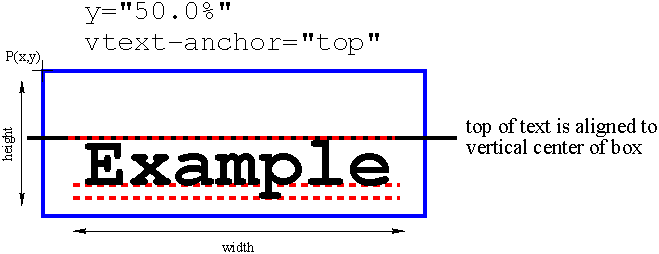
\includegraphics{figures/VerticalTextPlacement2.pdf}
\end{center}
\caption{vertical text alignment \token{top}}
\label{VerticalTextPlacement2}
\end{figure}

\subsubsection{Bottom}

\begin{figure}[h!]
\begin{center}
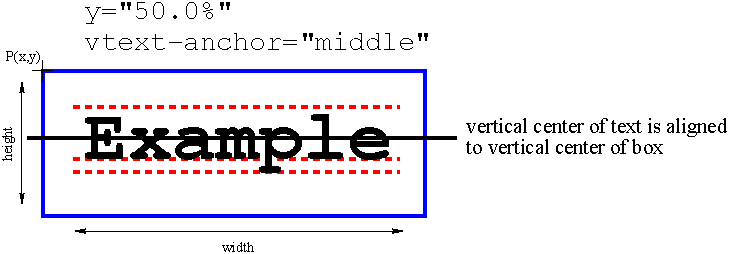
\includegraphics{figures/VerticalTextPlacement3.pdf}
\end{center}
\caption{vertical text alignment \token{bottom}}
\label{VerticalTextPlacement3}
\end{figure}

\clearpage

\subsubsection{Middle}

\begin{figure}[h!]
\begin{center}
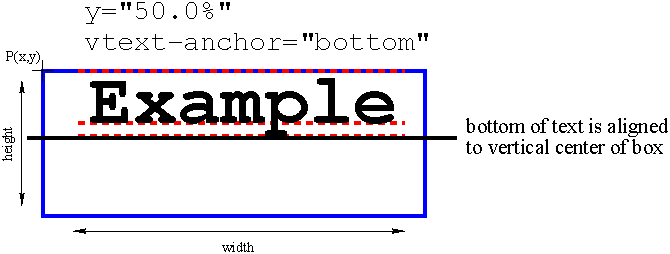
\includegraphics{figures/VerticalTextPlacement4.pdf}
\end{center}
\caption{vertical text alignment \token{middle}}
\label{VerticalTextPlacement4}
\end{figure}

\subsubsection{Baseline}

\begin{figure}[h!]
\begin{center}
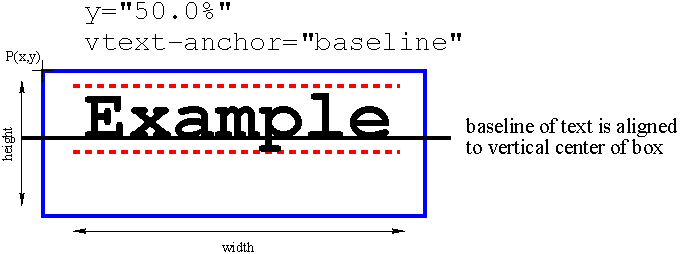
\includegraphics{figures/VerticalTextPlacement5.pdf}
\end{center}
\caption{vertical text alignment \token{baseline}}
\label{VerticalTextPlacement5}
\end{figure}

\clearpage

\subsection{Horizontal Text Anchor Examples}

The following figures illustrate the use of different \HTextAnchor values.

\subsubsection{Start}

\begin{figure}[h!]
\begin{center}
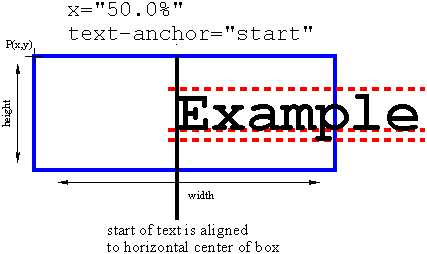
\includegraphics{figures/HorizontalTextPlacement_Start.pdf}
\end{center}
\caption{horizontal text alignment \token{start}}
\label{HorizontalTextPlacement_Start}
\end{figure}

\subsubsection{Middle}

\begin{figure}[h!]
\begin{center}
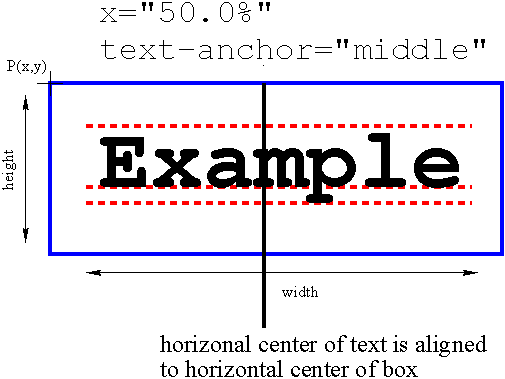
\includegraphics{figures/HorizontalTextPlacement_Middle.pdf}
\end{center}
\caption{horizontal text alignment \token{middle}}
\label{HorizontalTextPlacement_Middle}
\end{figure}

\clearpage

\subsubsection{End}

\begin{figure}[h!]
\begin{center}
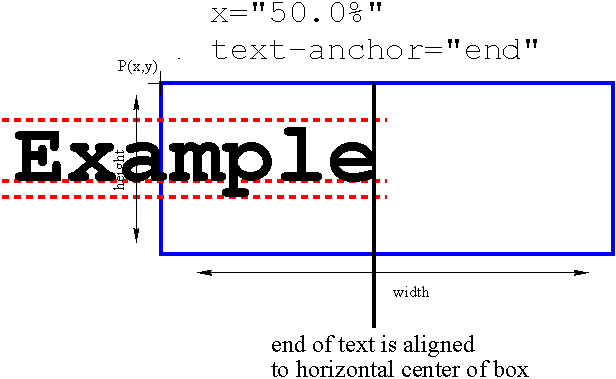
\includegraphics{figures/HorizontalTextPlacement_End.pdf}
\end{center}
\caption{horizontal text alignment \token{end}}
\label{HorizontalTextPlacement_End}
\end{figure}

